\documentclass{article}
\usepackage{amsmath}
\usepackage{graphicx}

\begin{document}



In recent years it has become clear that stellar mergers of all kinds of stars, main-sequence stars, post main sequence stars, and stellar remnants like white dwarfs and neutron stars are relatively common and play a central role in a wide variety of astrophysical phenomena. These include but are not limited to bright transients such as red novae, type Ia supernovae, and the birth of unusual stars that defy our understanding of stellar evolution, such as R Coronae Borealis stars, blue stragglers, and others. In the long run, better simulations of stellar mergers can improve our understanding of type Ia supernovae, which are key in cosmology, the origin of chemical elements, the origin of interacting binary stars, and stellar evolution.

Most stars form together as binary systems. Initially, the two stars will evolve separately from one another. Once the hydrogen fuel in the core of a star is burned, if the core contracts until its temperature is high enough to fuse helium, the star's outer layer expands, and the star evolves into a giant. This typically happens over billions of years. When a star in a binary system evolves into a giant, it may swallow up its companion. This is called the common envelope phase, and it may last millions of years. Eventually, the action of the smaller companion moving through the envelope will cause the envelope to heat up and dissipate as the orbit shrinks. When the second star evolves into a giant, a second common envelope phase may develop. It is also possible to form a "contact binary" in this phase, in which the two stars are touching one another. 

Typically as a binary's orbit shrinks, tidal forces will cause the spin of each star to increase so that each star's spin frequency matches the orbital frequency. If the system becomes small enough that its spin angular momenta exceeds 1/3 of its orbital angular momentum, an instability develops in which the components are not able to convert enough orbital momentum to spin momentum to remain tidally locked. This is called the Darwin instability. When this happens in a contact binary, the binary will merge to form a single star.

In 2008, a known contact binary, V1309 Sco, was observed to suddenly increase in brightness by a factor of 10 over hundreds of days (Tylenda et al., 2011). This eruption, known as a "red nova," was caused by the merger of the binary system. Based on observational constraints and evolutionary modeling, Stepien (2011) proposed four possible evolutionary tracks from the progenitor binary system to the system's state just before merge. Three of these tracks resulted in a primary of mass 1.52-1.54 $M_\odot$  and a secondary with mass 0.16-0.17 $M_\odot$.

We aim to use Octo-tiger to model a contact binary similar to the ones proposed by Stepien. The initial model is produced using the self-consistent field technique (SCF), and its parameters are chosen such that the spin angular momentum barely exceeds 1/3 of the orbital angular momentum. We will simulate the ensuing disruption and merger of the system and produce a light curve for comparison with the observed light curve of V1309. If we can reproduce the observed light curve, this would be a powerful validation of the Octo-tiger code.

\begin{figure}
\begin{center}
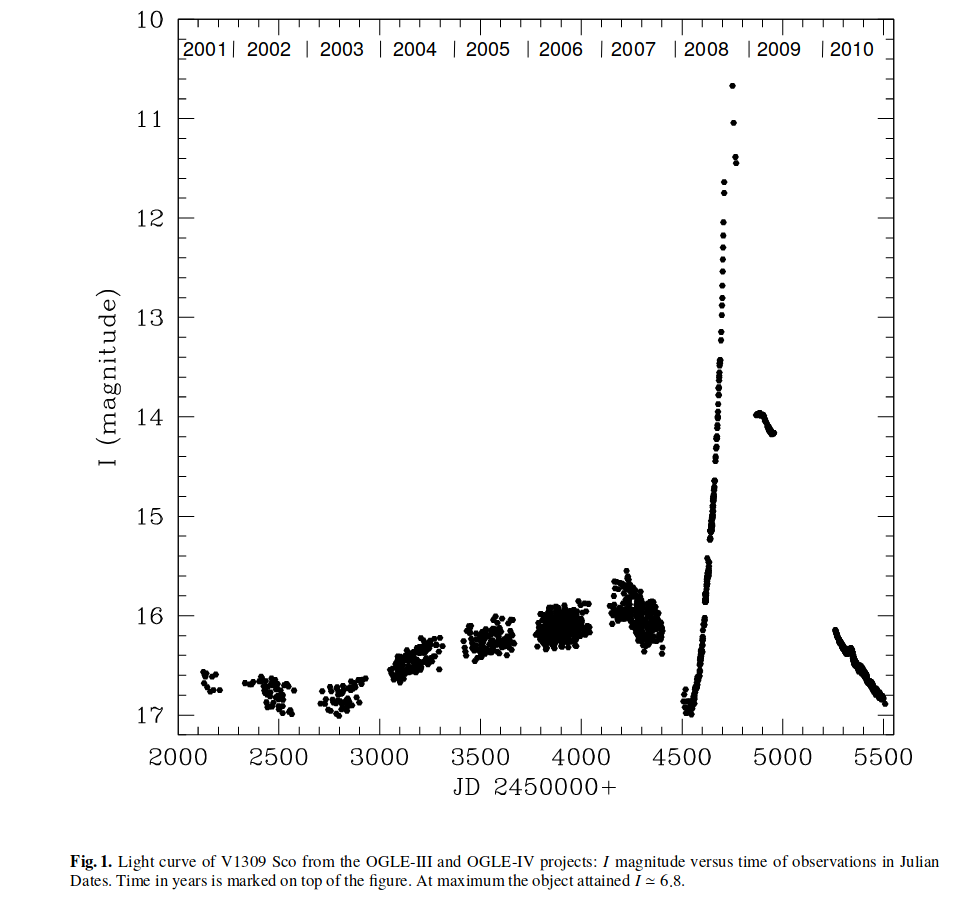
\includegraphics[width=1.25\textwidth]{fig1}
\end{center}
\caption{Reproduced from Tylenda et. al. 2011}
\end{figure}

\end{document}
